\documentclass[a4paper,12pt]{article}
\usepackage[bahasa]{babel}
\usepackage{graphicx}
\usepackage{multirow}
\usepackage{enumitem}
\usepackage{listings}
\usepackage{adjustbox}
\graphicspath{ {./img/} }
\begin{document}
\title{Laporan Praktikum Statistika Pertemuan 10}
%\author{Aldzikri Dwijayanto Prathama \\ {\small 195410189}}
\author{Aldzikri Dwijayanto Prathama 
	\\195410189}
\makeatletter
\begin{titlepage}
	\begin{center}
		{\huge \bfseries \@title }\\[14ex]
		
\includegraphics[scale=.8]{logo}\\[4ex]
		{\large \@author}\\[20ex]
		{\large \bfseries {SEKOLAH TINGGI MANAJEMEN INFORMATIKA DAN KOMPUTER
				AKAKOM YOGYAKARTA}}
	\end{center}


%{\large \@date} 
\end{titlepage}
\makeatother
%\maketitle
\newpage
\tableofcontents
\newpage
\section{Pembahasan}
Probabilitas adalah kemungkinan yang dapat terjadi dalam suatu peristiwa tertentu. Definisi probabilitas dapat dilihat dari tiga macam pendekatan, yaitu pendekatan klasik, pendekatan frekuensi relatif dan pendekatan subjektif.

\subsection{Praktik}
\subsubsection{Praktik 1}
Pada praktik 1 digunakan pendekatan klasik, menurut pendekatan klasik pada suatu peristiwa random dapat terjadi dalam n cara yang masing-masing memiliki kemungkinan yang sama, dan apabila sejumlah n(B) digunakan untuk cara memberikan hasil B.
\begin{center}
	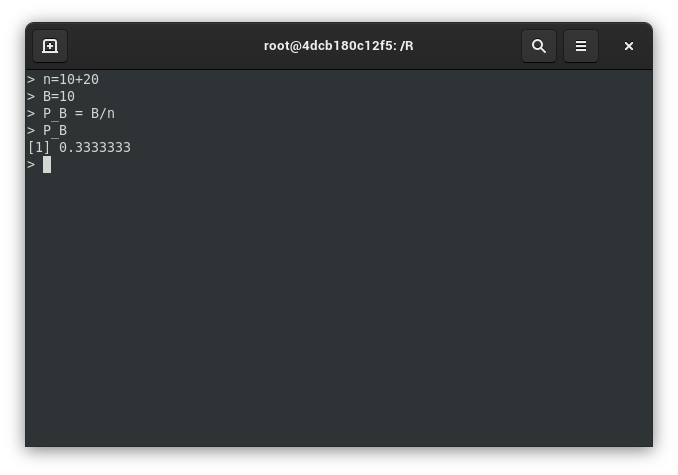
\includegraphics[scale=.5]{prak1}
\end{center}
Pada R Console kita ketikkan\\
\texttt{n=10+20}\\
artinya kita memberi nilai n dengan 10 butir telur bebek ditambah dengan 20 butir telur ayam yaitu 30 butir telur, kemudian klik enter. Selanjutnya kita ketikkan \\
\texttt{B=10}\\
artinya B adalah 10 butir telur. Kemudian kita beri rumus\\ 
\texttt{P\_B = B/n }, kemudian kita panggil lagi P\_B. Maka peluang terambil telur bebek adalah 0,33333. 
\end{document}